\documentclass[a4paper,12pt]{article}
% PDF-Metadaten
\pdfinfo{    
     /Title (PDF-Titel) 
     /Subject   (PDF-Thema)    
     /Author  (Vorname Nachname) 
     /Keywords   (Stichwort1,Stichwort2)      
} 
\usepackage[T1]{fontenc}
\usepackage[utf8]{inputenc}
\usepackage{lmodern}
% für Deutsche Begriffe und Silbentrennung
\usepackage[ngerman]{babel}
% required for equations
\usepackage{amsmath}
% required to include graphics
\usepackage{graphicx}
% Abkürzungsverzeichnis
\usepackage{acronym}
% Stichwortverzeichnis
\usepackage{makeidx}
\makeindex
% Zeilenabstand 1,5 Zeilen
\usepackage{setspace}
\onehalfspacing
% BibLaTeX benutzen
\usepackage[backend=biber,citestyle=alphabetic,bibstyle=alphabetic]{biblatex}
\addbibresource{Bibliographie.bib}
\DeclareLabelalphaTemplate{
  \labelelement{
    \field[final]{shorthand}
    \field{label}
    \field[strwidth=3,strside=left,ifnames=1]{labelname}
    \field[strwidth=1,strside=left]{labelname}
  }
\labelelement{
        \literal{-}
      }
  \labelelement{
    \field[strwidth=2,strside=right]{year}
  }
}
% Seitenränder anpassen
\usepackage{geometry}
\geometry{left=2cm, right=2cm, top=2.5cm, bottom=2cm}
\usepackage{epstopdf}

\title{My first \LaTeX{} document}
\author{Jon Doe}

\begin{document}

\newpage\null\thispagestyle{empty}\newpage
\newpage
\pagestyle{empty}

%\begin{figure}[t]
%	\centering
%	\includegraphics[width=0.6\textwidth]{Abb/logo_fbi}
%\end{figure}

\begin{center}
\Large Hochschule Darmstadt \\
\normalsize \textsc{- Fachbereich Maschinenbau und Kunststofftechnik -} \\

\vfill

\Huge Der Titel der Arbeit \\
\normalsize
\vspace{12pt}
Abschlussarbeit zur Erlangung des akademischen Grades \\ 
Bachelor of Science (B.Sc.) 

\vfill

vorgelegt von \\
Vorname Nachname

\vfill

\begin{tabular}[h]{p{4cm}l l}
	Referent(in): & Name des Erstbetreuers\\
	Korreferent(in):  & Name des Zweitbetreuers
\end{tabular}

\end{center}

\newpage
\pagestyle{plain}
\section*{Eidesstattliche Erklärung}
\addcontentsline{toc}{section}{Eidesstattliche Erklärung}
Ich versichere hiermit, dass ich die vorliegende Arbeit selbständig verfasst und keine
anderen als die im Literaturverzeichnis angegebenen Quellen benutzt habe. \\

\noindent Alle Stellen, die wörtlich oder sinngemäß aus veröffentlichten oder noch nicht veröffentlichten
Quellen entnommen sind, sind als solche kenntlich gemacht. \\

\noindent Die Zeichnungen oder Abbildungen in dieser Arbeit sind von mir selbst erstellt worden oder mit
einem entsprechenden Quellennachweis versehen. \\

\noindent Diese Arbeit ist in gleicher oder ähnlicher Form noch bei keiner anderen Prüfungsbehörde
eingereicht worden.
\newline\newline
Darmstadt, den \today
\newpage
\section*{Abstrakt}
\addcontentsline{toc}{section}{Abstrakt}
\newpage
\section*{Vorwort}
\addcontentsline{toc}{section}{Vorwort}
\newpage
\addcontentsline{toc}{section}{Inhaltsverzeichnis}
\tableofcontents
\newpage
\section{Einführung}
Lorem ipsum dolor sit amet, consectetur adipiscing elit \ac{KDE}. Donec a diam lectus \cite{Accardi.2010}. Sed sit amet ipsum mauris. \index{Maecenas} congue ligula ac quam viverra nec consectetur ante hendrerit \cite{Lewis.2010}. Donec et mollis dolor. Praesent et diam eget libero egestas mattis sit amet vitae augue. Nam tincidunt congue enim, ut porta lorem lacinia consectetur. 

\begin{figure}[h]
\center 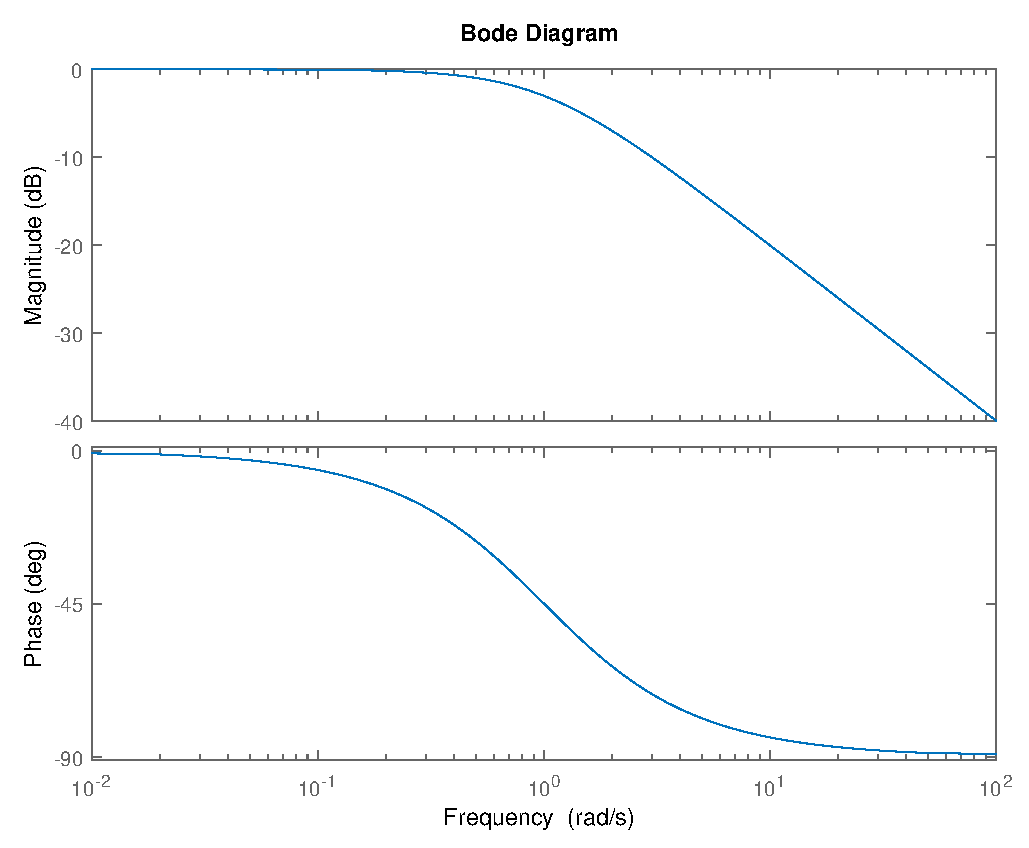
\includegraphics[width=0.5\textwidth]{Bilder/PT1/PT1.eps}
\caption{Bodediagramm PT1}
\end{figure}

\subsection{Motivation}
Donec ut libero sed arcu vehicula ultricies a non tortor. Lorem ipsum dolor sit amet, consectetur adipiscing elit. Aenean ut gravida lorem. Ut turpis felis, pulvinar a semper sed, adipiscing id dolor. Pellentesque auctor nisi id magna consequat sagittis. Curabitur dapibus enim sit amet elit pharetra tincidunt feugiat nisl imperdiet.

\begin{table}[h]
	\center
	\begin{tabular}[h]{|c|c|}
		\hline
		$U_e$ / V& $U_a$ / V\\ \hline
		0.1 & 0.2 \\ \hline
		0.2 & 0.4 \\ \hline
		0.3 & 0.6 \\ \hline
		0.4 & 0.8 \\ \hline
		0.5 & 1 \\ \hline
	\end{tabular}
	\caption{Messergebnisse}
\end{table}

Ut convallis libero in urna ultrices accumsan. Donec sed odio eros. Donec viverra mi quis quam pulvinar at malesuada arcu rhoncus. Cum sociis natoque penatibus et magnis dis parturient montes, nascetur ridiculus mus. In rutrum accumsan ultricies. Mauris vitae nisi at sem facilisis semper ac in est \cite{Pleisteiner.2007}.

\newpage
\addcontentsline{toc}{section}{Literatur}
\printbibliography
\newpage
\printindex
\newpage
\section*{Abkürzungsverzeichnis}
\addcontentsline{toc}{section}{Abkürzungsverzeichnis}
\begin{acronym}[Bash]
 \acro{KDE}{K Desktop Environment}
 \acro{SQL}{Structured Query Language}
 \acro{Bash}{Bourne-again shell}
 \acro{JDK}{Java Development Kit}
 \acro{VM}{Virtuelle Maschine}
 \acro{I2C}[IC]{Inter-Integrated Circuit}
\end{acronym}
\newpage
\addcontentsline{toc}{section}{Abbildungsverzeichnis}
\listoffigures
\newpage
\addcontentsline{toc}{section}{Tabellenverzeichnis}
\listoftables
\newpage
\section*{Anhang}
\addcontentsline{toc}{section}{Anhang}
\end{document}